\chapter{Results Analysis}\label{chap:results}
\section{Evaluation scope}
The experiments address three decisions at a charging location with limited history. The first is whether to initialize a forecaster from other locations. The second is how strongly to constrain the target encoder during adaptation. The third is whether to vary the contribution of two forecasters after observing their errors. Table~\ref{tab:res-scope} identifies the targets and comparison used for each decision.

\begin{table}[H]\centering\small
\caption{Target populations and initial histories.}\label{tab:res-scope}
\begin{tabular}{>{\raggedright\arraybackslash}p{.29\linewidth}>{\raggedright\arraybackslash}p{.36\linewidth}l}\toprule
Comparison & Target identifiers & History (days)\\\midrule
Backbone benchmark & 4 UrbanEV Development & 14\\
GRU initialization & 12 additional UrbanEV Development & 7, 14, 28\\
Coefficient calibration & 4 UrbanEV Development & 14\\
Historical selection and fusion & 90 selected across 7 dataset--city groups, Final partition & 7, 14, 28\\
Follow-up fusion evaluation & 46 additional Development IDs across 7 groups & 14\\
\bottomrule\end{tabular}
\end{table}

MAE measures the absolute error in hourly energy, in kWh. Lower values indicate better forecasts. Within a comparison, methods are scored on matched forecast origins with complete next-day observations. The historical comparison contains 21 groups from seven dataset--city groups crossed with three history budgets. One of the 90 selected identifiers had no scored outcome. Repeated seeds share target observations. The historical cohort was revisited during method development. The final comparison in this chapter uses a separately locked list of Development identifiers.

\clearpage
\section{Source transfer and backbone choice}
\subsection{Independent backbone benchmarks}
Two implementations evaluated models on the same four UrbanEV targets with 14 days of initial history. Table~\ref{tab:baselines} gives the mean error in each training mode. Bold marks the lowest MAE in each column. A dash denotes a mode without a reported result. Custom attention in A and official TimeXer in B \cite{wang2024timexer} are distinct architectures. The separate spatial benchmark uses histories from supporting locations. Its MAE is reported once per implementation.
\begin{table}[H]
\centering\small
\caption{Independent baseline MAE on four UrbanEV targets (kWh).}\label{tab:baselines}
\begin{tabular*}{\textwidth}{@{\extracolsep{\fill}}lrrrr@{}}\toprule
& \multicolumn{2}{c}{Implementation A} & \multicolumn{2}{c}{Implementation B}\\\cmidrule(lr){2-3}\cmidrule(l){4-5}
Model & Target only & Transfer & Target only & Transfer\\\midrule
Daily naive & 7.0763 & -- & 7.0757 & --\\
Weekly naive & 8.4631 & -- & 8.4631 & --\\
Ridge & 5.9339 & -- & 5.9339 & --\\
SARIMA & 6.5799 & -- & 6.6771 & --\\
Random forest & \textbf{5.8008} & -- & \textbf{5.8204} & --\\
XGBoost & 6.4847 & -- & 6.4613 & --\\
MLP & 8.6711 & 5.5196 & 8.6855 & 5.4753\\
GRU & 8.9406 & \textbf{5.3150} & 8.9239 & 5.3157\\
LSTM & 8.9360 & 5.3356 & 8.9565 & 5.3168\\
TCN & 8.0734 & 5.3447 & 7.8415 & 5.3027\\
Custom attention & 8.1209 & 5.5823 & -- & --\\
Official TimeXer & -- & -- & 7.0224 & \textbf{5.1979}\\
\midrule
GCN--LSTM (spatial) & \multicolumn{2}{c}{7.1288} & \multicolumn{2}{c}{7.1790}\\
\bottomrule\end{tabular*}
\end{table}

Random forest had the lowest target-only MAE in both implementations. With source initialization, GRU ranked first in A (5.3150 kWh), narrowly ahead of LSTM (5.3356). In B, TimeXer ranked first (5.1979), followed by TCN (5.3027) and GRU (5.3157). Across both implementations, all 60 paired neural model--entity--seed comparisons per implementation favored source initialization. The GRU provided a competitive backbone with 52,376 trainable parameters for the controlled retention experiments. The ranking applies to the training settings and four targets tested here.

\subsection{Transfer after calibrating the target training budget}
A target-only neural model may need more initial training than a pretrained one. We compared 3, 10, 30, 100 and 300 initial epochs on four calibration targets. The lowest calibration MAE occurred at 30, 100 and 100 epochs for target-only training with 7, 14 and 28 days of history, respectively. With source initialization, the corresponding values were 3, 3 and 10 epochs. We evaluated these settings on twelve additional targets. Both models used the same architecture and scored days. Source fine-tuning used zero latent penalty, so the comparison measures the benefit of starting from a source checkpoint under the separately calibrated budgets.


Figure~\ref{fig:budget-curves} shows why the two initialization modes received different training budgets. Open circles mark the lowest calibration MAE on each curve. Table~\ref{tab:res-transfer} reports the subsequent evaluation on twelve additional targets.
\begin{figure}[htbp]\centering
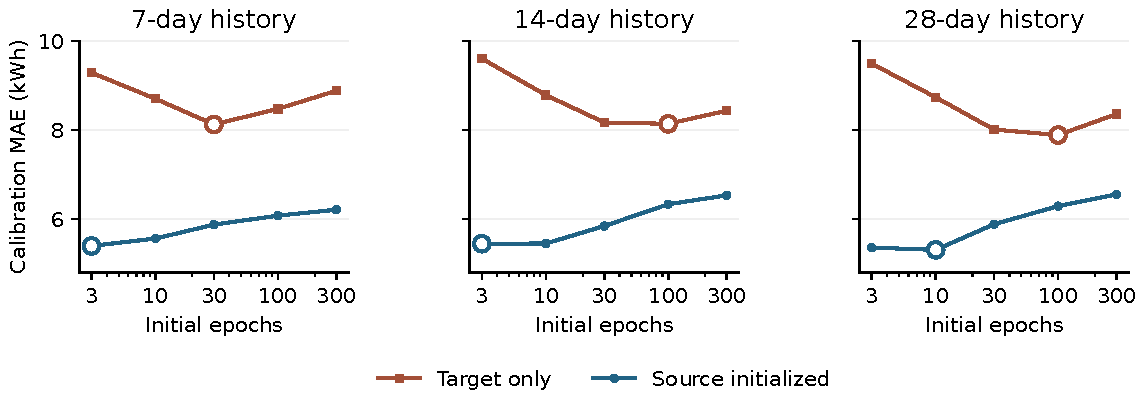
\includegraphics[width=.97\linewidth]{Images/budget-curves.pdf}
\caption{Initial training budget on four calibration targets.}\label{fig:budget-curves}
\end{figure}

\begin{table}[H]\centering\small
\caption{GRU initialization on twelve UrbanEV targets (MAE in kWh).}\label{tab:res-transfer}
\begin{tabular}{lrrr}\toprule
Initial history & Target-only MAE & Transfer MAE & Reduction\\\midrule
7 days & 5.0521 & \textbf{3.3671} & 33.35\%\\
14 days & 4.8341 & \textbf{3.3046} & 31.64\%\\
28 days & 4.7697 & \textbf{3.3482} & 29.80\%\\
\bottomrule\end{tabular}
\end{table}

At 14 days, for example, source initialization reduced mean error by 1.5295 kWh per hour (Table~\ref{tab:res-transfer}). The advantage persisted at 28 days despite allowing the target-only model 100 initial epochs. These reductions describe the mean over the selected UrbanEV targets at each budget. They provide a reason to retain source initialization when studying the smaller effects of regularization and online decisions. The four-target backbone benchmark also used a different source training budget (three epochs versus ten here), so its absolute MAEs should be interpreted within that benchmark.
\clearpage
\section{Fixed and adaptive retention}
\subsection{Measured retention strength on the calibration targets}
For each tested coefficient, the encoder gradient ratio compares the weighted retention gradient with the forecast gradient on the same parameters,
\begin{equation}
\rho=\frac{\|\lambda\nabla_{\theta_{\rm enc}}R\|_2}{\|\nabla_{\theta_{\rm enc}}F\|_2+10^{-12}}.
\end{equation}
\begin{table}[H]\centering
\caption{Representative fixed coefficients on four calibration targets.}
\small\begin{tabular}{lrrr}\toprule
Role & $\lambda$ & Median $\rho$ & MAE (kWh)\\\midrule
Zero reference & 0 & 0 & 5.443630\\
Forecast-dominated, higher MAE & 0.000390 & 0.000922 & 5.444004\\
Forecast-dominated, lower MAE & 0.474980 & 0.559958 & 5.361266\\
Calibration minimum & 0.798445 & 0.792279 & \textbf{5.331706}\\
Retention-dominated, lower MAE & 8.163598 & 7.234187 & 5.371132\\\bottomrule
\end{tabular}
\end{table}
Among the twenty positive coefficients, five had a median gradient ratio below one and a higher calibration MAE than zero retention. Ten had a ratio below one and a lower MAE. The other five had a ratio above one and a lower MAE. Each representative row illustrates an observed combination of gradient strength and error direction relative to zero. These classifications apply at the sampled points. The calibration minimum is shown separately.

\begin{figure}[H]\centering
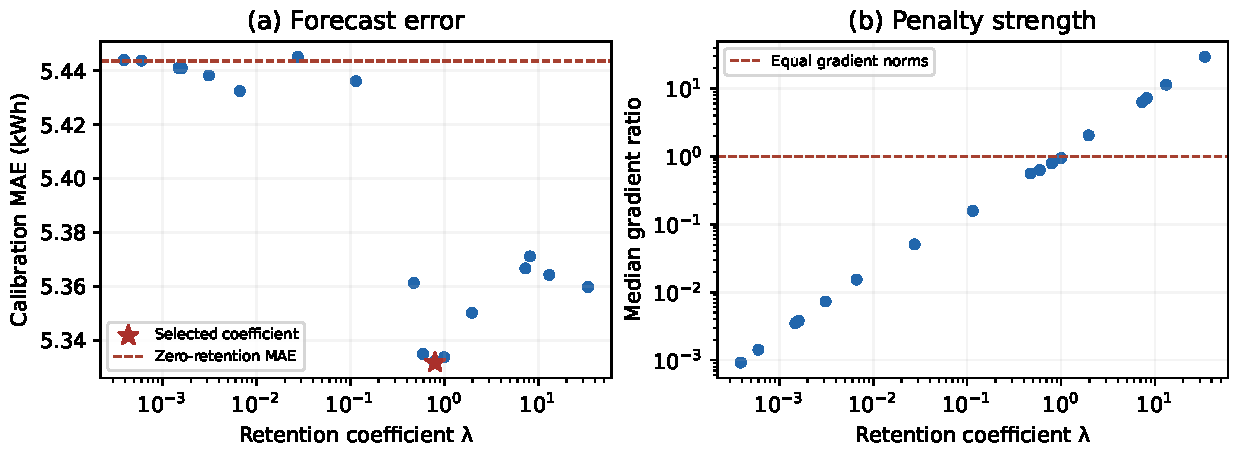
\includegraphics[width=.95\linewidth]{Images/fixed-evidence.pdf}
\caption{Calibration error and encoder gradient ratios.}\label{fig:res-fixed}\end{figure}

Figure~\ref{fig:res-fixed} plots the 20 positive coefficients on a logarithmic axis. The dashed lines mark zero-retention MAE in (a) and equal gradient norms in (b). The selected coefficient reduced calibration MAE by 0.111925 kWh.

\subsection{Does switching retention reduce forecast error?}
The historical selector could switch among three coefficients after a completed block. The candidates used $\lambda\in\{0,0.1,1\}$. Its comparator held $\lambda=1$. Figure~\ref{fig:res-selector} compares the percentage reduction in group MAE against Fixed and Online-best. Positive values favor switching. Against Fixed, all three histories favored switching in CHARGED/MEL, SPO and SZH, giving nine wins. All three favored Fixed in UrbanEV/SZH, AMS, JHB and LOA. Against Online-best, which selects by past error without a confidence gate, the historical confidence rule yielded lower MAE in eleven of 21 groups. In each comparison all eighteen finite exploratory intervals included zero. The three UrbanEV intervals were undefined in each comparison.

\begin{figure}[H]\centering
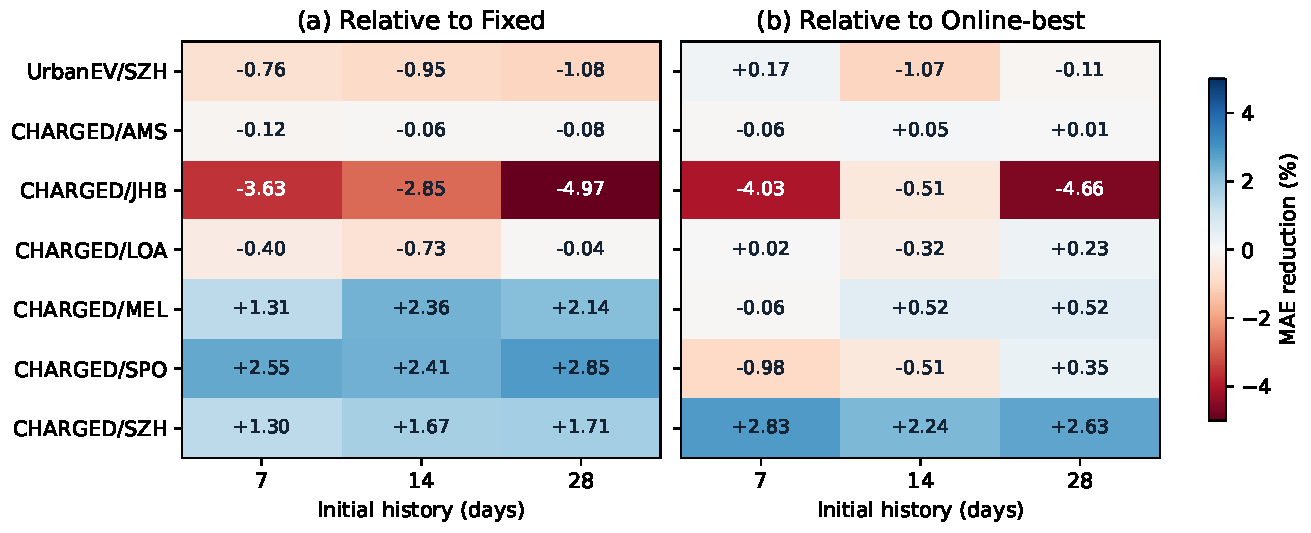
\includegraphics[width=\linewidth]{Images/selector-gains.pdf}
\caption{Historical retention switching versus Fixed and Online-best.}\label{fig:res-selector}\end{figure}

The \href{https://github.com/HungLD9505/adaptive-retention-ev/blob/52a91d3/report/full-results.csv}{historical results by group} give both contrasts for each history. The twelve-target Development study used a different control. Its fixed trajectory was selected on calibration targets and then compared with two selectors drawing on the same bank of independent trajectories. The past-MAE rule selected using past errors, while the confidence rule required evidence for switching.

\begin{table}[H]\centering\small
\caption{Selection from a common bank on twelve targets (MAE in kWh).}\label{tab:res-bank}
\begin{tabular}{lrrr}\toprule
History & Calibrated Fixed & Past MAE & Confidence rule\\\midrule
7 days & \textbf{3.3186} & 3.3234 & 3.3234\\
14 days & \textbf{3.2670} & 3.2904 & 3.2755\\
28 days & 3.3482 & 3.3252 & \textbf{3.3140}\\
\bottomrule\end{tabular}
\end{table}

The confidence rule improved on calibrated Fixed only at 28 days, where calibration had selected zero retention (Table~\ref{tab:res-bank}). At seven days the two selectors agree to four decimal places.

On the four previously inspected calibration targets, a separate experiment allocated the first 28 scheduled days to calibration, two to an embargo and the final 60 to evaluation. The embargo days remained part of causal replay. The four targets contributed 60, 22, 22 and 22 scored days in that final window, with equal weight per target after averaging seeds. Discrete selection reached 4.7983 kWh, calibrated Fixed 4.8031 and continuous selection 4.8062. Continuous exceeded Fixed by 0.00317 kWh. The discrete method used three branches and a different initialization and tuning budget, so this comparison cannot isolate the effect of coefficient continuity.

A separate \href{https://github.com/HungLD9505/adaptive-retention-ev/blob/52a91d3/docs/reports/issue99-decision-probe-20261110/handoff.md}{one-step decision experiment} cloned the current state before an update and compared following the continuous controller with holding its coefficient. Following reduced the next forecast error in 153 of 294 paired forecasts. The equal-target mean difference (follow minus hold) was $-0.000182$ kWh on these previously inspected calibration targets. In the persistent-shadow calibration, one of 57 completed decisions accepted a proposed change, from 69 proposals overall. Its mean MAE reduction against Fixed was 0.000118 kWh. Neither diagnostic establishes a practically useful decision threshold.


Figure~\ref{fig:issued-lambda} shows the coefficient recorded at each issued forecast for all four targets and all three seeds. Each point denotes an issued forecast; gaps indicate days without one. The dashed horizontal line marks the calibrated Fixed coefficient. These trajectories show how much the controller moved; the later-window MAEs above measure the forecasting consequence.
\begin{figure}[htbp]\centering
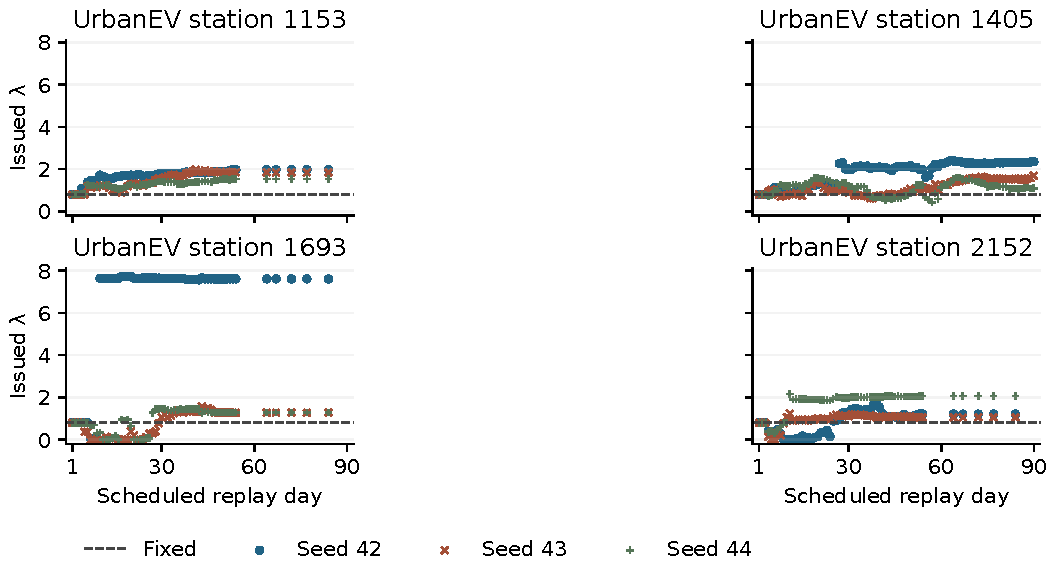
\includegraphics[width=.97\linewidth]{Images/issued-lambda.pdf}
\caption{Continuous retention coefficients at issued forecasts.}\label{fig:issued-lambda}
\end{figure}

\section{Combining two forecasts and adapting their weights}
The stable and fast GRUs differ in retention strength and in the history used for online updates. Static and adaptive fusion combine the same two forecast streams. Comparing either with single Fixed measures the overall change from using two experts. Comparing adaptive with static isolates the effect of updating their weights.

\begin{figure}[H]\centering
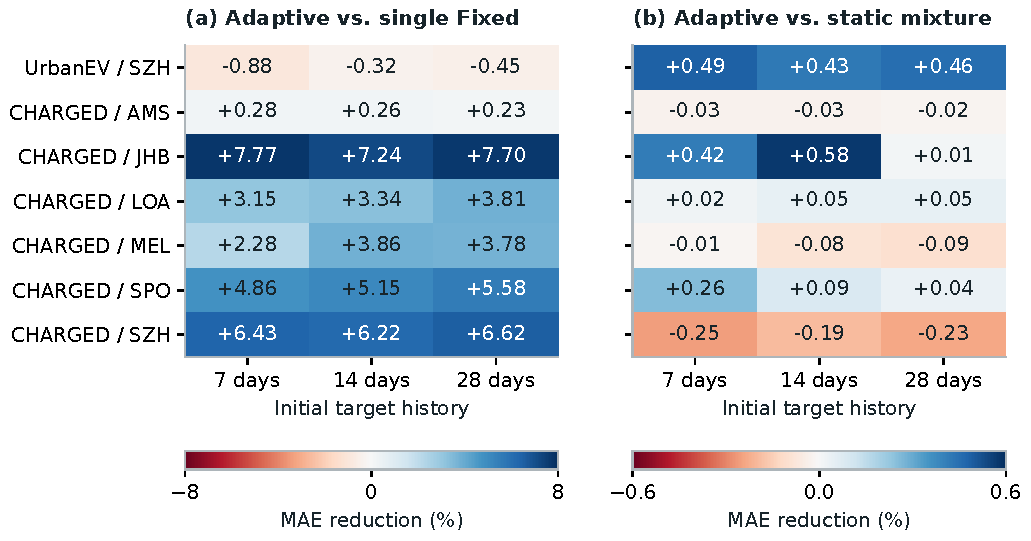
\includegraphics[width=.95\linewidth]{Images/cohort-comparisons.pdf}
\caption{Historical fusion gains. Color limits are $\pm8\%$ against Fixed and $\pm0.6\%$ against static fusion.}\label{fig:res-fusion}\end{figure}

Both mixtures improved on single Fixed in 18 of 21 historical groups. Adaptive fusion reduced MAE in all eighteen CHARGED groups (0.23--7.77\%) and increased it in all three UrbanEV groups (0.32--0.88\%). In the matched comparison, adaptive weights improved on static weights in twelve groups and increased error in nine. The panels in Figure~\ref{fig:res-fusion} use separate scales because the weighting differences are smaller.

At 14 days in UrbanEV/SZH, adaptive weighting improved the static mean from 8.0361 to 8.0016 kWh, yet single Fixed reached 7.9758. In CHARGED/MEL, adaptive fusion reached 52.2649 kWh compared with 54.3655 for single Fixed and 52.2222 for static fusion. The two examples show why a win count depends on the control. Posthoc resampling across entities gave intervals spanning zero in thirteen of the 21 adaptive-versus-static comparisons.

\clearpage
\subsection{Examples across forecast dates}

\begin{figure}[H]\centering
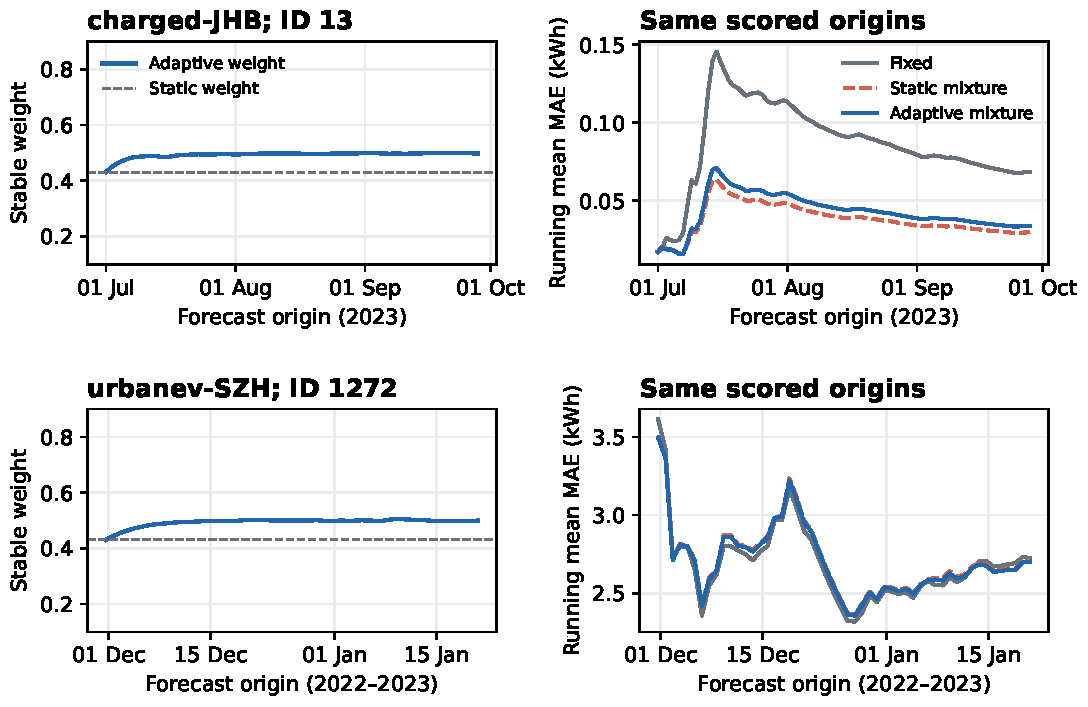
\includegraphics[width=.95\linewidth]{Images/trajectories.pdf}
\caption{Historical expert weights and running mean daily errors at two targets.}\label{fig:res-traces}\end{figure}

Figure~\ref{fig:res-traces} follows JHB identifier 13 and UrbanEV identifier 1272 at 14 days with seed 42. Within each group, the selection rule used the upper median of the entity-level gains against Fixed among targets with Fixed MAE above $10^{-4}$ kWh. The displayed seed illustrates the trajectory. Target selection used gains averaged across seeds. Weights at each forecast origin use only feedback available by that time. The running mean divides the sum of daily MAEs by the number of scored origins to date. Each trace illustrates one target, while the group comparisons average over targets and seeds.

A bounded follow-up on the twelve Development targets at 14 days compared alternative weight updates. AdaHedge \cite{rooij2014} reduced MAE from 3.291048 to 3.284880 kWh relative to the original adaptive rule. Single Fixed achieved 3.267000 kWh, so the alternative did not meet its criterion for further evaluation.

\clearpage
\section{Evaluation on additional Development targets}
The follow-up fixed both controls, the forecast recipe and the 46 target identifiers before evaluating their outcomes. At the 14-day budget, 3,948 of 4,140 scheduled identifier--day pairs had complete outcomes. These targets came from the same seven dataset--city groups and evaluation calendar, so the follow-up tests performance on additional identifiers within that setting. Table~\ref{tab:res-confirm} shows group MAE in kWh and percentage reductions relative to each control. Bold marks the lowest MAE in each row.

\begin{table}[H]\centering\small
\caption{Forecast errors on the 46 additional Development identifiers.}\label{tab:res-confirm}
\resizebox{\linewidth}{!}{\begin{tabular}{@{}lrrrrrrr@{}}\toprule
Group & IDs & Fixed & Fast & Static & Adaptive & vs Fixed (\%) & vs static (\%)\\\midrule
UrbanEV/SZH & 10 & \textbf{7.4023} & 8.8496 & 8.1106 & 7.9944 & -8.00 & +1.43\\
CHARGED/AMS & 10 & 16.2823 & \textbf{16.2107} & 16.2287 & 16.2344 & +0.29 & -0.03\\
CHARGED/JHB & 1 & 8.0410 & 8.4356 & 7.9544 & \textbf{7.9147} & +1.57 & +0.50\\
CHARGED/LOA & 10 & 2.0621 & 2.1082 & 2.0371 & \textbf{2.0317} & +1.48 & +0.26\\
CHARGED/MEL & 4 & \textbf{10.9073} & 11.6425 & 11.1002 & 11.0267 & -1.10 & +0.66\\
CHARGED/SPO & 1 & 8.4985 & \textbf{7.6644} & 7.7956 & 7.8368 & +7.79 & -0.53\\
CHARGED/SZH & 10 & 4.2698 & 4.3512 & 4.1675 & \textbf{4.1578} & +2.62 & +0.23\\
\bottomrule\end{tabular}}
\end{table}

Adaptive fusion improved on single Fixed in five of seven groups and on static fusion in five of seven. The groups differed between comparisons. In UrbanEV/SZH, it reduced error by 1.43\% against static fusion but increased it by 8.00\% against Fixed. In SPO, it reduced error by 7.79\% against Fixed and increased it by 0.53\% against static. SPO and JHB each contributed one identifier, so each of those group means describes a single target.

Figure~\ref{fig:locked-intervals} shows both primary intervals on the same scale. Positive values favour adaptive fusion.
\begin{figure}[htbp]\centering
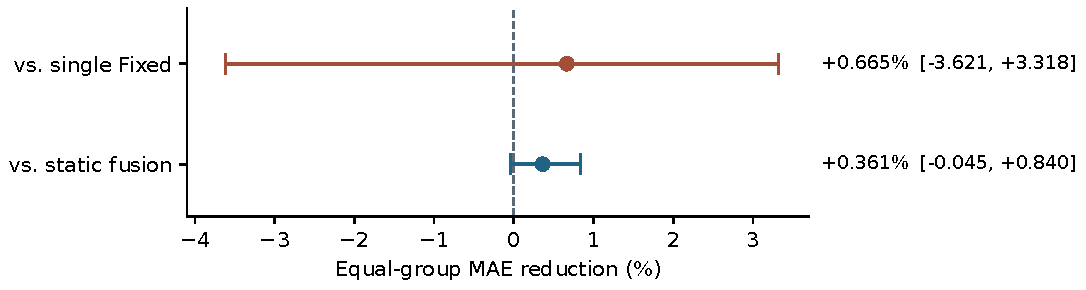
\includegraphics[width=.97\linewidth]{Images/locked-intervals.pdf}
\caption{Adaptive fusion on 46 targets: estimates and nominal 97.5\% intervals.}\label{fig:locked-intervals}
\end{figure}

Giving each dataset--city group equal weight, adaptive fusion reduced MAE by 0.6653\% relative to single Fixed and 0.3610\% relative to static. 

The paired resampling analysis gave nominal 97.5\% intervals of $[-3.6209,3.3176]\%$ and $[-0.0449,0.8399]\%$, respectively. The prespecified criterion required both lower bounds to exceed zero. The prespecified three-day sensitivity intervals also included zero. At fourteen days each comparison had two undefined replicates out of 10,000, leaving both sensitivity intervals undefined. Both primary intervals include zero, so the evaluation did not establish superiority to both controls. The more consistent empirical finding across the chapter is the benefit of source initialization under short target histories. The added benefit of adapting retention or forecast weights depends on the target group and the comparator.
